\section{Date: 2026-11-24}
\noindent \textbf{Series ID: IEAXSTC} 

\noindent This series is titled Exports of Services: Telecommunications, computer, and information services and has a frequency of Quarterly. The units are Millions of Dollars and the seasonal adjustment is Seasonally Adjusted.The observation start date is 1999-01-01 and the observation end date is 2026-04-01.The popularity of this series is 3. \\ 

\noindent \textbf{Series ID: COLATZ315} 

\noindent This series is titled Import Price Index by Origin (NAICS): Apparel Manufacturing for Latin America and has a frequency of Monthly. The units are Index Jun 2012=100 and the seasonal adjustment is Not Seasonally Adjusted.The observation start date is 2012-06-01 and the observation end date is 2026-10-01.The popularity of this series is 2. \\ 

\subsection{Raw Regression}
\noindent Regresses the two series against each other directly. A significant result here can come just as easily from both series sharing a long-run trend as from any real relationship.

\begin{center}
\begin{tabular}{lclc}
\toprule
\textbf{Dep. Variable:}       & value\_fred\_COLATZ315 & \textbf{  R-squared:         } &     0.587   \\
\textbf{Model:}               &          OLS           & \textbf{  Adj. R-squared:    } &     0.579   \\
\textbf{Method:}              &     Least Squares      & \textbf{  F-statistic:       } &     75.20   \\
\textbf{Date:}                &    Tue, 24 Nov 2026    & \textbf{  Prob (F-statistic):} &  9.61e-12   \\
\textbf{Time:}                &        21:38:33        & \textbf{  Log-Likelihood:    } &   -126.03   \\
\textbf{No. Observations:}    &             55         & \textbf{  AIC:               } &     256.1   \\
\textbf{Df Residuals:}        &             53         & \textbf{  BIC:               } &     260.1   \\
\textbf{Df Model:}            &              1         & \textbf{                     } &             \\
\textbf{Covariance Type:}     &       nonrobust        & \textbf{                     } &             \\
\bottomrule
\end{tabular}
\begin{tabular}{lcccccc}
                              & \textbf{coef} & \textbf{std err} & \textbf{t} & \textbf{P$> |$t$|$} & \textbf{[0.025} & \textbf{0.975]}  \\
\midrule
\textbf{const}                &      92.8981  &        1.008     &    92.154  &         0.000        &       90.876    &       94.920     \\
\textbf{value\_fred\_IEAXSTC} &       0.0005  &     6.33e-05     &     8.672  &         0.000        &        0.000    &        0.001     \\
\bottomrule
\end{tabular}
\begin{tabular}{lclc}
\textbf{Omnibus:}       &  7.131 & \textbf{  Durbin-Watson:     } &    0.282  \\
\textbf{Prob(Omnibus):} &  0.028 & \textbf{  Jarque-Bera (JB):  } &    6.385  \\
\textbf{Skew:}          &  0.651 & \textbf{  Prob(JB):          } &   0.0411  \\
\textbf{Kurtosis:}      &  4.044 & \textbf{  Cond. No.          } & 4.88e+04  \\
\bottomrule
\end{tabular}
%\caption{OLS Regression Results}
\end{center}

Notes: \newline
 [1] Standard Errors assume that the covariance matrix of the errors is correctly specified. \newline
 [2] The condition number is large, 4.88e+04. This might indicate that there are \newline
 strong multicollinearity or other numerical problems.

\begin{figure}
\centering
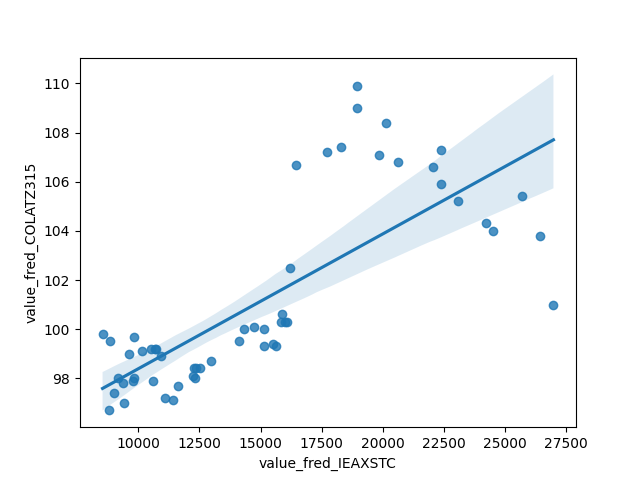
\includegraphics[scale = 0.9]{plots/plot_2026-11-24.png}
\caption{Raw Regression Plot for 2026-11-24}
\end{figure}
\newpage
\subsection{Detrended Regression}
\noindent Regresses the residuals of each series after removing its own linear time trend, so a shared trend can no longer drive the result on its own. A relationship that stays significant here is better evidence of a genuine link between the two series.

\begin{center}
\begin{tabular}{lclc}
\toprule
\textbf{Dep. Variable:}                  & value\_fred\_COLATZ315\_detrended & \textbf{  R-squared:         } &     0.006   \\
\textbf{Model:}                          &                OLS                & \textbf{  Adj. R-squared:    } &    -0.013   \\
\textbf{Method:}                         &           Least Squares           & \textbf{  F-statistic:       } &    0.2990   \\
\textbf{Date:}                           &          Tue, 24 Nov 2026         & \textbf{  Prob (F-statistic):} &    0.587    \\
\textbf{Time:}                           &              21:38:33             & \textbf{  Log-Likelihood:    } &   -124.34   \\
\textbf{No. Observations:}               &                   55              & \textbf{  AIC:               } &     252.7   \\
\textbf{Df Residuals:}                   &                   53              & \textbf{  BIC:               } &     256.7   \\
\textbf{Df Model:}                       &                    1              & \textbf{                     } &             \\
\textbf{Covariance Type:}                &             nonrobust             & \textbf{                     } &             \\
\bottomrule
\end{tabular}
\begin{tabular}{lcccccc}
                                         & \textbf{coef} & \textbf{std err} & \textbf{t} & \textbf{P$> |$t$|$} & \textbf{[0.025} & \textbf{0.975]}  \\
\midrule
\textbf{const}                           &   -3.655e-13  &        0.319     & -1.15e-12  &         1.000        &       -0.639    &        0.639     \\
\textbf{value\_fred\_IEAXSTC\_detrended} &       0.0001  &        0.000     &     0.547  &         0.587        &       -0.000    &        0.001     \\
\bottomrule
\end{tabular}
\begin{tabular}{lclc}
\textbf{Omnibus:}       &  4.335 & \textbf{  Durbin-Watson:     } &    0.266  \\
\textbf{Prob(Omnibus):} &  0.114 & \textbf{  Jarque-Bera (JB):  } &    3.777  \\
\textbf{Skew:}          &  0.641 & \textbf{  Prob(JB):          } &    0.151  \\
\textbf{Kurtosis:}      &  3.063 & \textbf{  Cond. No.          } & 1.35e+03  \\
\bottomrule
\end{tabular}
%\caption{OLS Regression Results}
\end{center}

Notes: \newline
 [1] Standard Errors assume that the covariance matrix of the errors is correctly specified. \newline
 [2] The condition number is large, 1.35e+03. This might indicate that there are \newline
 strong multicollinearity or other numerical problems.

\begin{figure}
\centering
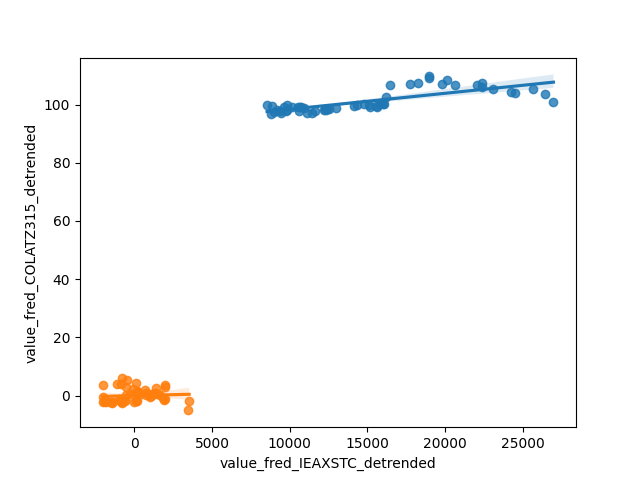
\includegraphics[scale = 0.9]{plots/plot_2026-11-24_detrended.png}
\caption{Detrended Regression Plot for 2026-11-24}
\end{figure}
\newpage
